\documentclass[a4paper,10.5pt]{article}
\usepackage{mathtools}
\usepackage{listings}
\usepackage{tikz-qtree}

\usepackage[utf8x]{inputenc}
\usepackage[font=small,format=plain,labelfont=bf,up,textfont=normal,up]{caption}
\usepackage[left=2.2cm,top=2cm,right=2.2cm,bottom=2cm,nohead,nofoot]{geometry}
\usepackage{wrapfig}
\usepackage{graphicx}
\usepackage{subcaption}
\setlength{\footskip}{25pt}
\usepackage{tikz}
\usepackage{amsmath,tikz}
\usetikzlibrary{shapes.geometric}
\usepackage{subcaption}
\usepackage{pgfplots}
\usepackage{filecontents}
\usepackage{algpseudocode}
\usepackage{algorithm}
\usepackage{subfig}
\usepackage{float}
\usepackage{graphicx}
\usepackage{marginnote}
\usepackage{pgfgantt}
\usepackage{pdflscape}
\usepackage{wrapfig}
\usepackage{tikz}

\usepackage{forest}
\usepackage{tikz-qtree}

\usepackage{listings}
\usepackage{color}
\usepackage{pgfplots}
\usepackage{filecontents}
\pgfdeclarelayer{background}
\usetikzlibrary{matrix}
\usetikzlibrary{shapes,arrows}

\definecolor{mygreen}{rgb}{0,0.6,0}
\definecolor{mygray}{rgb}{0.5,0.5,0.5}
\definecolor{mylightgray}{HTML}{F2F2F2}
\definecolor{mymauve}{rgb}{0.58,0,0.82}

\lstset{ language=C,
  backgroundcolor=\color{mylightgray},   % choose the background color; you must add \usepackage{color} or \usepackage{xcolor}
showstringspaces=false,
belowcaptionskip=0em,
    belowskip=-1em,
  basicstyle=\footnotesize,        % the size of the fonts that are used for the code
  breakatwhitespace=false,         % sets if automatic breaks should only happen at whitespace
  breaklines=true,                 % sets automatic line breaking
  captionpos=b,                    % sets the caption-position to bottom
  commentstyle=\color{mygreen},    % comment style
  deletekeywords={...},            % if you want to delete keywords from the given language
  escapeinside={\%*}{*)},          % if you want to add LaTeX within your code
  extendedchars=true,              % lets you use non-ASCII characters; for 8-bits encodings only, does not work with UTF-8
  frame=single,                    % adds a frame around the code
  keepspaces=true,                 % keeps spaces in text, useful for keeping indentation of code (possibly needs columns=flexible)
  keywordstyle=\color{blue},       % keyword style
  language=Octave,                 % the language of the code
  morekeywords={*,...},            % if you want to add more keywords to the set
  numbers=left,                    % where to put the line-numbers; possible values are (none, left, right)
  numbersep=5pt,                   % how far the line-numbers are from the code
  numberstyle=\tiny\color{mygray}, % the style that is used for the line-numbers
  rulecolor=\color{white},         % if not set, the frame-color may be changed on line-breaks within not-black text (e.g. comments (green here))
  showspaces=false,                % show spaces everywhere adding particular underscores; it overrides 'showstringspaces'
  showstringspaces=false,          % underline spaces within strings only
  showtabs=false,                  % show tabs within strings adding particular underscores
  stepnumber=0,                    % the step between two line-numbers. If it's 1, each line will be numbered
  stringstyle=\color{mymauve},     % string literal style
  tabsize=2,                       % sets default tabsize to 2 spaces
  title=\lstname                  % show the filename of files included with \lstinputlisting; also try caption instead of title
}

\renewcommand{\footnoterule}{%
  \kern -3pt
  \hrule width \textwidth height 0.5pt
  \kern 2pt
}
\tikzstyle{decision} = [diamond, draw, fill=white!20, 
    text width=6em, text badly centered, node distance=3cm, inner sep=1pt]
\tikzstyle{block} = [rectangle, draw, fill=white!20, 
    text width=5em, text centered, rounded corners, minimum height=3em]
\tikzstyle{line} = [draw, -latex']
\tikzset{
  treenode/.style = {align=center, inner sep=0pt, text centered,
    font=\sffamily},
 arn_n/.style = {treenode, circle, white,  font=\sffamily, draw=black,
    fill=black, text width=1.5em}
}
\usepackage{marginnote}
\usepackage{pgfgantt}
\usepackage{rotating}
\usepackage{pdflscape}
\usepackage{float}
\title{Random Number Generation Using Genetic Programming\\ {\large BSc Computer Science Dissertation}}
\author{{\small by}\\\\Philip Leonard}

\tikzset{
    maxfitnessorgen /.style={
        /pgfplots/execute at end plot visualization={\draw [current plot style, dashed] (@auxnode.center) -- ($(@auxnode.center)!10cm!(@auxnode.east)$);}
    },
    maxfitnessorgen nodestyle/.style={
        pos=1, inner sep=0pt, sloped, alias=@auxnode
    }
}
\definecolor{lblue}{HTML}{33B5E5}
\definecolor{lgrey}{HTML}{7F8C8D}
\definecolor{lpurple}{HTML}{AA66CC}
\definecolor{lgreen}{HTML}{99CC00}
\definecolor{lorange}{HTML}{FFBB33}
\definecolor{lred}{HTML}{FF4444}
\definecolor{dblue}{HTML}{0099CC}
\definecolor{dpurple}{HTML}{9933CC}
\definecolor{dgreen}{HTML}{669900}
\definecolor{dorange}{HTML}{FF8800}
\definecolor{dred}{HTML}{CC0000}

\pgfplotscreateplotcyclelist{androidstyle}{
{dblue},
{lred},
{lorange},
{lgreen},
{lpurple},
{dorange},
{lgrey},
}

\pgfplotscreateplotcyclelist{androidstyle2}{
{lblue},
{lred},
}

\begin{filecontents}{sngpreduced.dat}
a b
10 0
20 60
40 60
60 70
80 80
100 80
\end{filecontents}

\begin{filecontents}{gpreduced.dat}
a b
50 0
100 40
200 40
300 20
400 40
500 40
\end{filecontents}

\begin{filecontents}{cvsmyrand.dat}
a b c
10 0.000000 0.000000
100 0.000000 0.000000
1000 0.002000 0.000000
10000 0.026000 0.001000
100000 0.235000 0.004000	
1000000 2.400000 0.044000	 		
10000000 24.085001 0.477000
100000000 236.805008 4.573000
\end{filecontents}

\begin{filecontents}{cvsmyrandc.dat}
a b
10 0.000000
100 0.000000
1000 0.000000
10000 0.001000
100000 0.004000	
1000000 0.044000	 		
10000000 0.477000
100000000 4.573000
1000000000 46.348999
10000000000 463.489990
\end{filecontents}

\begin{filecontents}{rand_runtime.dat}
a b c
10 0.010000 0.000000
100 0.016000 0.000000	
1000 0.023000 0.000000
10000 0.030000 0.001000	
100000 0.037000 0.001000	
1000000 0.043000 0.001000	
10000000 0.054000 0.001000
\end{filecontents}

\begin{document}
\maketitle

\begin{abstract}
This is the final report for the project; `Random Number Generation Using Genetic Programming' by Philip Leonard, supervised by Dr David Jackson (primary supervisor) and Professor Paul Dunne (secondary supervisor). This document covers all aspects of the project from the introduction and background, to the design implementation and analysis of the project in order to give the reader an understanding of how I implemented the project and what things I found when evaluating the project.

This report demonstrates that using methods described by Koza in \cite{kozarng}, it is possible to genetically breed Random Number Generators that produce sequences of pseudo random bits with near maximal entropy. This report more importantly shows that it is possible to produce better results using the Single Node Genetic Programming methodology described by Jackson in \cite{jacksonsngp}. As well as this, this report also demonstrates that the Random Number Generators Produced genetically by these methods also produce sequences of random bits with higher entropy than other widely used RNGs. It not only outperforms the C programming Linear Congruent Generator algorithm implemented in the $rand()$ function, but can also perform better than a Hardware / ``True" Random Number Generator that creates random bit sequences from observed atmospheric noise.\newline

\noindent \textbf{Keywords:} Genetic Algorithm (GA), Genetic Programming/Program (GP), Pseudo Random Number Generator (PRNG), Random Number Generator (RNG), True Random Number Generator (TRNG), Entropy, Single Node Genetic Programming/Program (SNGP), Crossover, Mutation, Fitness proportionate reproduction (FPR), Linear Congruent Generator (LCG).
\end{abstract}

\newpage

\tableofcontents
\newpage
\section{Introduction}
%Whats a RNG?
Random Number Generators have many computational, scientific and societal applications. They are essential in; gambling, lottery draws, cryptography, statistical sampling, Monte Carlo simulations and other applications where and unpredictable result is desired. Randomness can be interpreted in more than one way and has no strict mathematical definition. There are a series of tests that can be run on a set of data in order to evaluate some conception of randomness. These include the gap test, frequency test, runs test and information entropy test amongst others described in the NIST\footnote{National Institute of Standards and Technology} ``\emph{Test Suite for Random and Pseudorandom Number Generators for Cryptographic Applications}" \cite{nist}. Whilst there isn't a way to prove randomness, these statistical tests are a good way of analysing randomness in the eyes of the user and for their practical application. In this project, randomness is tested using the Shannon Entropy equation \cite[p.2]{kozarng}, which is a measure of the unpredictability/uncertainty in a random variable.
A Pseudo Random Number Generator (PRNG) is a program/algorithm which generates numbers that possess the characteristics of a ``truly" random number. These programs typically employ seed values (an example being the number of nanoseconds since the Unix epoch\footnote{00:00:00 (UTC), Thursday, 1 January 1970}), or they use a sequence of consecutive numbers as an input. Mathematical operations are applied to this input in order to fabricate a ``random" number or bit sequence. This differs from true random number generators which typically use a piece of hardware to measure an unpredictable environmental occurrence such as radiation, measured by a Geiger Counter. 

%What is Genetic Programming - EXPAND ON THIS
The Genetic Programming paradigm is an evolutionary method of solving problems, where the implementer can define a task where solutions can be randomly generated and tested by some fitness function. The population can then be evolved based on their fitness in order to search through the problem space to find solutions which meet the fitness requirements of the implementer. 
Inspired by Evolutionary Algorithms, Genetic Programming is a method used to evolve computer programs using the Darwinist theory of natural selection (survival of the fittest). The general framework for Genetic Programming is;
\begin{description}
  \item[1)]
  \ \ To begin with, a random initial population of computer programs (traditionally in a tree structure) is generated from a set of functions/operators and terminals. 
  \item[2)]
 \ \ \ A fitness function is used to assess the fitness of each program, i.e. how well the program does it's job, or how accurate the computed output is. 
  \item[3)]
  \ \ \ Genetic operations such as crossover and mutation are used in order to generate new offspring programs.
  \item[4)]
 \ \ \ The fitness of the new population is then assessed again, and the programs for the next generation are then selected.
\end{description}
The process from steps three and four are then repeated, creating new generations of ``fitter" programs. Generally, Genetic Program runs terminate when a member of the population reaches a certain pre-defined fitness, or when the run has reached a certain number of generations. Fitness functions, probabilities and genetic operations all vary from problem to problem.

%Aim of the Project
Evolving Random Number Generators is therefore an applicable problem instance for Genetic Programming, as there is no deterministic way of producing a RNG with high entropy.  The aim of the project is to assess two Genetic Programming methodologies in order to determine which is best suited for genetically breeding RNGs. The method described by Koza in \cite{kozarng} was followed in order to implement the idea of evolving a random number generator in the widely known traditional Genetic Programming methodology. The next step was to implement the same idea using the Single Node Genetic Programming Methodology described by Jackson in \cite{jacksonsngp}. The effectiveness of both where then compared by gathering data from both implementations and conducting some cross examination to determine the victor. In order to determine the effectiveness of the Random Number Generators as a real world solution, entropy data was gathered from pre-existing and widely used RNGs. These were namely the C rand function, which is a Pseudo Random Number Generator which is makes use of a Linear Congruent Generator algorithm in order to produce random numbers, and a ``True" Random Number Generator was also evaluated in order to compare the effectiveness of the genetically produced RNGs against a non-deterministic source of random data. 

%Challanges of the project?
Attempting to match Koza's implementation was a one of the major challenges of the project. Koza doesn't give many details of how he implemented the Genetic Program. Instead he gives a theoretical overview of the operations, and then the results of his implementation. Therefore a good understanding of the GP paradigm template was required in order to take Koza's words and implement them successfully as a working program. 

%Solutions produced?
In terms of software three programs have been produced. The GP implementation and the SNGP implementation form two separate single threaded command line programs. The command line interface displays information and run progress to the user, and all data for each generation and each run, including entropy values and is written to log files. 
The third program developed is to test both the C random number generator and the TRNG and to write the entropy data to log files as well.
From these implementations I was then able to start to collect data. In order to gather sufficient data for analysis, I ran both the SNGP and GP implementations 50 times and also ran 50 tests of the C rand funtion and the TRNG. 

%Effectivness of solution.
The effecitvness of the solution can be viewed in two ways. To begin with, both methods are viable ways to produce RNGs by evolutionary means. Therefore the implemented software was a succesfull venture. The other and perhaps more important evaluation of how effective the solutions are is whether the SNGP proves a more effective way of producing RNGs than GP, and wether they stand up to other widely used RNGs (both deterministic and non-deterministic). The results of project are very promising. To begin with, SNGP proves a much faster way of evolving RNGs, finding solutions on average over 6 times quicker than the standard GP methodology. Not only is it quicker, but it also has a solution rate twice that of the Genetic Programming Methodology. The solutions produced by SNGP are also much smaller than those produced by GP, as branches can be repeated but there values can be stored and therefore only calculated once and stored dynamically. The solutions produced by the two genetic methodologies also outperformed the C rand function and even the ``True" Random Number Generator. 

\newpage
\section{Background}
%Introduce Koza's paper to explain the GP implementation. 
This project is based on two pieces of research into Genetic Programming from two separate research papers. The first paper by Koza entitled ``Evolving a Computer Program to Generate Random Numbers Using the Genetic Programming Paradigm" is the main basis for the project. It describes how Random Number Generators can be evolved using Genetic Programming. Koza describes the design for the implementation, and displays his results and findings. Koza concludes that it is possible to genetically breed randomisers with high entropy. The aim of the first part of this project was to take this implementation design and implement it in the C programming language, in order to try and match his results and outcomes. 

%Introduce Jacksons paper.
The second paper used to support this project is Jacksons paper entitled ``A New, Node-Focused Model for Genetic Programming" \cite{jacksonsngp}, where he introduces a new Genetic Programming paradigm known as Single Node Genetic Programming. Instead of using a population of tree structures like that of traditional GP, SNGP uses a graph population, where every node in the graph represents the root of a tree in it's own right. In this paper, Jackson introduces the SNGP model, and evaluates it's performance over a number of test cases which he also implemented in the GP paradigm. Jackson shows that SNGP outperforms GP in terms of solution rate, speed (efficiency) and the size of the solutions produced. The aim of the second part of this project is to further prove SNGPs computational superiority over the standard GP paradigm, again using the basis of evolving a RNG introduced by Koza in \cite{kozarng}, in order to create a SNGP variant of the same problem.

%Talk comparitively about the GP implementation to Koza's.
After implementing the GP variant of generating RNGs by evolutionary means, I was able to step back and compare the reults I had obtained to that of Koza's. As stated previously, trying to obtain the same results as Koza in \cite{kozarng} was one of the main challanges of the project. I was able to acheive individuals solutions with fitness/entropy that matched the fittest that Koza produced in \cite[p.6]{kozarng} of 27.996 out of 28.00 maximal bits of entropy. In general, the number of generations required to find solutions were greater in my implementation as opposed to the results produced by Koza. All other observations made by Koza however matched the ones I obtained from my implementation. For example, Koza explains that in the run that generated his fittest solution; \emph{``entropy reached and slowly improved within the 27.800 to 27.900 area"}. In all runs of my implementation I observed the same phenomenon of the GP implementation struggling to obtain the last 0.1 bits of entropy, and in fact is where most runs spent a large number of generations searching. I also obtained similar sized solutions Koza's results.

%Research needed and books read.
As discussed in the specification and design documents, research was the dominating factor in preparing for this project. I began researching Genetic Algorithms \cite[p.1 - 24]{mitchell} and Genetic Programming \cite[p.1 - 35]{introgp} \cite[p.73 - 191]{kozagpbook} topics. I then researched more specifically into Genetic Programming, including a C implementations of Multiplexer Problem described in \cite{kozamux}. The focal point of my research has been around the papers by Koza \cite{kozarng}, which is the inspiration for the implementation of this project using GP, and Jackson \cite{jacksonsngp2}. In \cite{kozarng}, Koza conducts some tests of the genetically produced RNGs against RNGs that were widely used at the time\footnote{Koza's paper was published in 1991}. I also felt that to show the success of the RNGs produced by GP and SNGP in my implementations, I should do the same. I therefore did some research current widely used RNGs today. I chose the C $rand()$ function as a comparative PRNG, and also a ``True" Random Number Generator, specifically from the random.org website. Seeing as the TRNG generates numbers by non-deterministic means, I felt it was a strong opponent to test against the (deterministic) PRNGs produced by evolutionary means.
%Project Requirements
The requirements for this project can be defined by 4 main objectives;
\begin{description}
  \item[1)]
  \ \ \ Replicate the program described by Koza in \cite{kozarng}, in the C programming language. 
  \item[2)]
 \ \ \ Deliver the same idea, but by using the Single Node Genetic Programming paradigm as described by Jackson in \cite{jacksonsngp2}, again as a C program.
  \item[3)]
  \ \  Deliver an analysis and a conclusion of the best method of genetically breeding a randomiser.
   \item[4)]
  \ \  Produce a final program testing the entropy of the C $rand()$ function and the TRNG at random.org, and deliver an analysis of the best practical method of producing random numbers.
\end{description}

\newpage
\section{Design}

%- Discuss how not using OO approach. How for GP and SNGP will each only require a single C program file.\\

In this section we discuss the design of the project. As the design document produced for this project provides a full overview of the design, in this section we shall take a look at the most important elements of the design, and the changes which have been made since that document was produced. For further details on the design, the full document can be found in the appendix at the end of this report. 
%- Discuss the anticipated components of the software\\
\subsection{GP Approach}
This section covers the design for the GP approach of evolving a RNG. 

The goal is to genetically breed a RNG to randomise a sequence of binary digits. The input to the RNG will be the sequence $J$, which will run from $i = 1$ to $2^{14}$. The output will be a sequence of random binary digits of size $J$. The binary digit at location $i$ will be determined by the value of the LSB\footnote{Least Significant Bit. The lowest (furthest right) bit in a binary sequence determining whether the number is odd or even.} from the output of the RNG on the $i^{th}$ input.

\begin{wrapfigure}{r}{.4\textwidth}
\caption{RNG binary tree}
\label{fig:simplebintree}
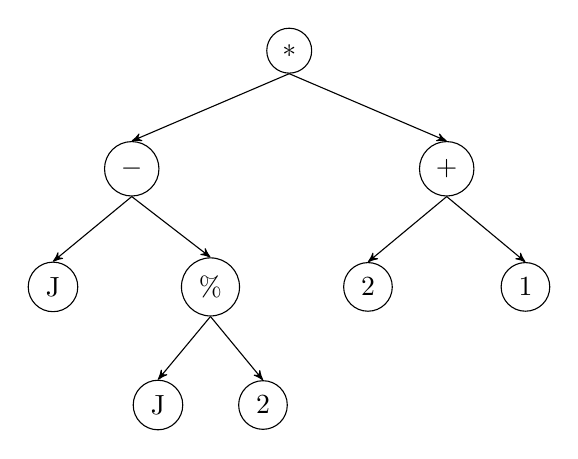
\begin{tikzpicture}[->,>=stealth',level/.style={sibling distance = 4cm/#1,
  level distance = 1.5cm}] 
\node[circle,draw](z){$*$}
 child{
    node[circle,draw]{$-$} child{node[circle,draw] {J}} child{node[circle,draw] {$\%$} child{node[circle,draw] {J}}  child{node[circle,draw] {2}}} }
  child{
    node[circle,draw]{$+$} child{node[circle,draw] {2}} child{node[circle,draw] {1}} };
\end{tikzpicture}
\end{wrapfigure}

As explained in \cite[p.19-27]{introgp} to begin designing a GP, the first step is to define the set of terminals and the set of functions, of which the program trees will be comprised of. The terminal set will be; \begin{center}$T = \{J,\ \Re\}$\end{center} $J$ as already discussed will be the value in the sequence 1 to $2^{14}$, and $\Re$ will represent a small random integer constant from the set $\{0, 1, 2, 3\}$. The set $F$ is our function or operator set; \begin{center}$F = \{+, -, *, /, \%\}$\end{center}In this set, $/$ is the protected integer quotient function and $\%$ is the protected modulus function, where both use the protected division function that returns 1 when attempting to divide by zero, and otherwise returns the normal quotient. All the terminals have an arity of 0, and all the functions have an arity of 2.

\begin{text}The next step is to define the structure of the programs. Members of the population will be represented as binary trees, in the form of prefix expressions. Take for example the expression; \end{text}
\begin{equation*}*\ -\ J\ \%\ J\ 2\ +\ 2\ 1 \end{equation*} 
This prefix expression can be represented as the binary tree in figure \ref{fig:simplebintree}. And vice versa, the prefix expression above can be generated from a pre-order traversal of the binary tree in figure \ref{fig:simplebintree}. For experimentation, the user will initially define the major parameters of the GP run. These parameters are defined in figure \ref{inputparam} below;

\begin{figure}[H]
\centering
\caption{Input parameters}
\label{inputparam}
\begin{tabular}{l*{6}{l}r}
Data Type             & Input description\\
\hline
Integer & Population size\\
Integer & Maximum number of generations\\
Integer & Maximum initial program depth and maximum crossover program depth\\
Double & Fitness proportionate reproduction to crossover operation balance\\
Double & Internal to external node crossover probabilities\\
Double & Target fitness value\\
\end{tabular}
\end{figure}

Now we have defined the parameters, the terminals $T$, the functions $F$, and the structural representation of the programs, the next step for the GP is to use these definitions to enumerate an initial random population of programs.

Defined by the user, the GP will generate a population of the given size, where each program in the population has a maximum initial tree depth of the given size. In order to generate a wide and genetically diverse initial population, in \cite[p.11-14]{introgp} Koza suggests the even combination of both ``grow" and ``full" methods to generate program trees known as the ``ramped half and half method". This allows for a range of tree shapes and sizes all the way from a single terminal node program such as $J$, all the way up to a program which would be produced by the full function. Using this ramped half and half method, we can obtain half a population of large programs, and another half of programs with varying shapes and sizes.

Now that the GP has obtained an initial random population, it will evaluate each program and calculate it's corresponding fitness. A discussed above, the output of the RNG is a sequence of random binary digits of length $J$. To calculate the output, we must run through the sequence $J$ from $I = 1$ to $2^{14}$ substituting the occurrences of $J$ in the program with $i$. The LSB of the output given $J = i$ corresponds to the value in the binary sequence at position $i$. The GP will then calculate the binary output sequence for each RNG in the population. 

Now that the GP has evaluated every RNG, it must use a fitness function to calculate the fitness for each RNG given its respective output. In order to measure how ``random" the output is from a RNG, their are a variety of statistical and mathematical techniques at our disposal as discussed earlier. In this case, we are going to use the Shannon entropy equation from the field of Information Theory as our fitness function. The entopy of a sequence of binary digits is the equality in the occurrence of a set of binary subsequences of length $h$ in that sequence. The Shannon entropy calculation for all possible $2^h$ binary subsequences of length $h$ is;
\begin{equation*}
E_{h} = - \sum_{j} P_{(hj)}\ \log_2\ P_{(hj)}
\end{equation*}
Here $j$ ranges over all possible subsequences of length $h$ in the binary sequence (the RNG output in this case). In order to achieve maximum entropy for $E_h$, all probabilities for all $2^h$ binary sub sequences of length $h$ must be equal to $\frac{1}{2^h}$.

To calculate the entropy for the output of every RNG, we want to evaluate it for more than one binary sub sequence length. This is achieved by calculating the summation of the formula above for $E_h$ but over a range of lengths of $h$ from 1 to $N_{max}$; 

\begin{equation*}
E_{total} = \sum_{h = 1}^{N_{max}} \left[ - \sum_{j} P_{(hj)}\ \log_2\ P_{(hj)} \right]
\end{equation*}
The maximum possible entropy value for sub sequences from 1 to $N_{max}$ can be calculated using the following sum;
\begin{eqnarray*}
E_{max} &=& \sum_{i = 1}^{N_{max}} i
\\ &=& \frac{N_{max}(N_{max} + 1)}{2}
\\ &=& \frac{7 \cdot (7 + 1)}{2}
\\ &=& 28
\end{eqnarray*}
In this GP implementation, We shall be using sub sequences of lengths 1 to 7, so $N_{max} = 7$. This will give us the maximum entropy and therefore the maximum fitness of 28.

Now that the fitness function has been defined. The entropy for every RNG's output is calculated, for sub sequences of lengths 1 to 7.
In the C implementation, each program (RNG) will be stored in an individual struct. Each struct will contain; the RNG code/prefix expression, the program length, the output binary sequence, the scalar entropy break down for each of the sub sequence lengths of $h$ from 1 to $N_{max} = 7$ and the total fitness (the sum of these scalar entropies). So far in the design, all of these pieces of information have been defined. The population of all these structs are contained in another ``population struct" of the size defined by the user. Representing the programs and the population like this allows for easy manipulation and portability between methods in the GP.

Figure \ref{simpleflow} is a simple flow chart representation for the GP. At this point we have defined the first 3 operations. The 4th step is a Boolean decision which determines the continuation or termination of the GP, based on one or both of the two following termination criteria being satisfied;
\begin{description}
  \item[1)]
  \ \ \ The program in the population with the maximum fitness/entropy is greater than or equal to the user defined target fitness value, or
  \item[2)]
 \ \ \ The current generation number is equal to the user defined maximum number of generations.
\end{description}

If neither of these criteria are met, then the next stage is to prepare a modified population for the next generation. If one or both of these criteria are met, the GP will terminate. Regardless of which outcome happens, data is gathered for that particular run and is saved to a text file in the format of a CSV\footnote{Where values are delimited using commas i.e. $w,\ x,\ y,\ z, ...$}(Comma Separated Values) file. Each output and it's type are defined in figure \ref{outputparam} below;

\begin{wrapfigure}[30]{h}{.4\textwidth}
\caption{GP flowchart}
\label{simpleflow}
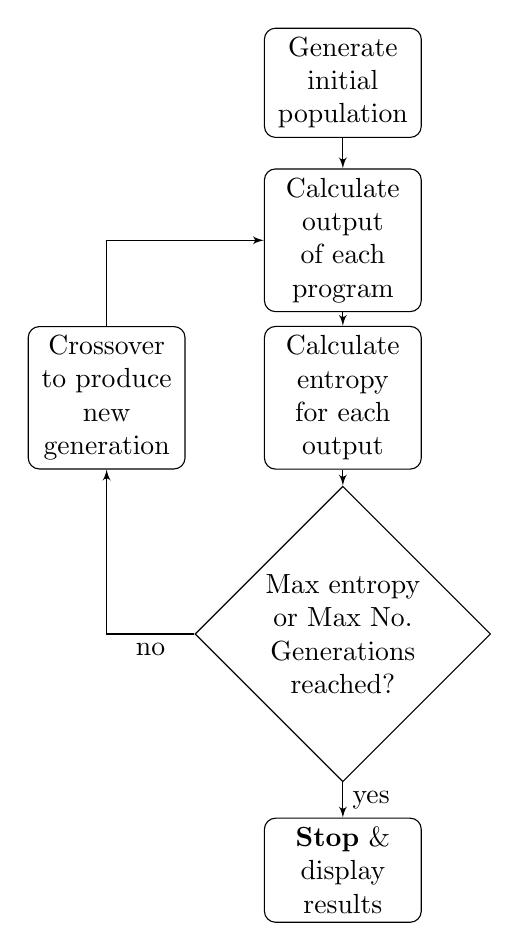
\begin{tikzpicture}[node distance = 2cm, auto]
    % Place nodes
    \node [block] (init) {Generate initial population};
    \node [block, below of=init] (identify) {Calculate output of each program};
    \node [block, below of=identify] (evaluate) {Calculate entropy for each output};
    \node [block, left of=evaluate, node distance=3cm] (update) {Crossover to produce new generation};
    \node [decision, below of=evaluate] (decide) {Max entropy or Max No. Generations reached?};
    \node [block, below of=decide, node distance=3cm] (stop) {\textbf{Stop} \& display results};
    % Draw edges
    \path [line] (init) -- (identify);
    \path [line] (identify) -- (evaluate);
    \path [line] (evaluate) -- (decide);
    \path [line] (decide) -| node [near start] {no} (update);
    \path [line] (update) |- (identify);
    \path [line] (decide) -- node {yes}(stop);
\end{tikzpicture}
\end{wrapfigure}


\begin{figure}[]
\centering
\caption{Output data}
\label{outputparam}
\begin{tabular}{l*{6}{l}r}
Data Type             & Output description\\
\hline
Integer & Generation number\\
Double & Generation run time in seconds \& hundredths of a second \\
Double & Average entropy/fitness for the population\\
Double & Total entropy/fitness of fittest candidate\\
Double & Entropy for subsequence size 1 of fittest candidate\\
\ \ \ \ $\vdots$ & \ \ \ \ \ \ \ \ \ \ \ \ \ \ \ \ \ \ \ \ \ \ \ \ $\vdots$\\
Double & Entropy for subsequence size 7 of fittest candidate\\
Boolean & Entropy of fittest candidate is $\geq$ target fitness?\\
String & Prefix expression for fittest candidate\\
\end{tabular}
\end{figure}


Since the design document, I have added in one extra piece of output data. This is the ``Average entropy/fitness for the population", and I included it so that during the analysis phase, I could determine how well the fitness of the population as a whole was growing and not just a single candidate. This comma separated data will be appended to the text file for each generation of the GP (each preceded with a return line character). For further information about the design of the structure of the output data, please refer to the design document in the appendix.

The final process in the GP to define is the genetic operation which shall be used. Two main genetic operations used in GP are mutation and crossover \cite[p.15-17]{introgp}. Both operate by altering program trees in different ways in order to create offspring programs. In this GP, I will be using the subtree crossover operation alone, and I will not be implementing subtree mutation in order to conserve computing time\footnote{Subtree mutation requires the generation of new subtrees which can prove to be computationally intensive, especially when mutation probability is high}.  

Subtree crossover works by taking two parent program trees and joining them to create two offspring programs. This is done by selecting a crossover point (node) in each parent tree. Both of the subtrees at the root of the crossover point are then swapped to generate the two new offspring. Crossover point selection can be at any node in the tree including leaf (in this case terminal) nodes. For this GP, one of the user inputs to the program in figure \ref{inputparam} on page \pageref{inputparam} is the probability divide of selection of internal to external nodes. In \cite[p.114]{kozagpbook}, Koza describes the benefits of using a 90\% internal (function) and 10\% external (terminal) split, saying that it ``promotes the recombining of larger structures" so that simple swapping of terminals like that of point mutation is less probable.

In figure \ref{inputparam} on page \pageref{inputparam}, there is a parameter ``Fitness proportionate reproduction to crossover operation balance". This input determines the split between Fitness proportionate reproduction (FPR) and crossover.  FPR is where both parents are selected for crossover relative to their fitness. In the regular crossover selection, one of the parents is selected relative to their fitness and the other is selected with an equal probability amongst the rest of the population. The following equation calculates the selection probability for the $i^{\text{th}}$ individual in the population (used for selecting both parents in FPR and one in crossover);\\
\begin{center}
\noindent\begin{minipage}{.3\linewidth}
\begin{equation*}
p_i = \Bigg( \frac{f_i}{\sum_{x=1}^{|P|} f_x} \Bigg)
\end{equation*}
\end{minipage}%
\begin{minipage}{.2\linewidth}
where;
\end{minipage}
\begin{minipage}{.3\linewidth}
$p_i$ - selection probability of $i$\\
$f_i$ - fitness value of $i$\\
$f_x$ - fitness value of $x$\\
$|P|$  - population size
\end{minipage}
\end{center}
Now that the GP has generated a new \emph{evolved} population, it returns back to step 2 in figure \ref{simpleflow} on page \pageref{simpleflow}. This process continues until one or both of the termination criteria are met as discussed above.

Above is a literal design of the GP, covering all the major aspects of the operations. Using the definitions above, a pseudocode can be created for the key methods in figure \ref{simpleflow} on page \pageref{simpleflow} which bears a closer functional resemblance to the actual C implementation of the GP. All algorithms produced in the design process can be found in the design document. Here I only introduce the changes made and the new algorithms introduced after the design document was written. 

In algorithm \ref{fitnessfunc} we can see that a minor change has been made since the design document was written. Instead of using a brute force pattern mactching algorithm, I have for the efficient finite automaton based KMP pattern matching algorithm (Named after it's designers, Knuth, Morris and Pratt). Algorithms \ref{prefixfunc} and \ref{kmpalgo} describe the two functions of this algorithm. The Compute-Prefix-Function creates a finite automaton transition function for the pattern that it is given. In essence this function calculates the earliest place in the pattern where the pattern can reoccur in itself. This way time is saved matching what has already been matched. The matching algorithm itself feeds the pattern through this automaton, keeping track of what state it is.

\begin{algorithm}[H]
  \caption{Compute-Prefix-Function$(j_2)$}
  \textbf{Input:} Binary pattern $j_2$.\\
  \textbf{Output:} The finite automaton mapping function $\pi$.\\
  \begin{algorithmic}[1]
	\State $m \gets $length($j_2$)
	\State $\pi[1] \gets 0$
	\State $k \gets 0$
	\For {$q \gets 2$ to $m$}
		\While {$k > 0 \land P[k + 1] \neq P[q]$}
			\State $k \gets \pi[k]$
		\EndWhile
		\If {$P[k + 1] == P[q]$}
			\State $k \gets k + 1$
		\EndIf
		\State $\pi[q] \gets k$
	\EndFor
	\State \textbf{return} $\pi$ \Comment {This algorithm returns the function $\pi$ where $\pi[q] = $max$\{k: P_k$ is a proper suffix of $P_q\}$}

  \end{algorithmic}
\label{prefixfunc}
\end{algorithm}

\begin{algorithm}[H]
  \caption{KMP-Matching$(j_2, O)$}
  \textbf{Input:} Binary pattern $j_2$ and the text (in this case binary sequence) $O$.\\
  \textbf{Output:} The number of occurrences of $j_2$ in $O$.\\
  \begin{algorithmic}[1]
  	\State $n \gets $length($O$)
	\State $m \gets $length($j_2$)
	\State $\pi \gets $Compute-Prefix-Function($j_2$)
	\State $q \gets 0$
	\State $count \gets 0$
	\For {$i \gets 1$ to $n$}
		\While {$q > 0 \land P[q + 1] \neq T[i]$}
			\State $q \gets \pi[q]$ \Comment{Using the prefix function to find the closest move backwards in the pattern we can go}
		\EndWhile
		\If {$P[q + 1] == T[i]$}
			\State $q \gets q + 1$
		\EndIf
		\If {$q == m$} \Comment {Reached the end of the pattern and therefore have a match}
			\State $count += 1$ 
			\State $q \gets \pi[q]$
		\EndIf
	\EndFor
	\State \textbf{return} $count$		 

  \end{algorithmic}
\label{kmpalgo}
\end{algorithm}

\begin{algorithm}[H]
  \caption{Fitness-Function($O$)}
  \textbf{Input:} Tree binary sequence output $O$\\
  \textbf{Output:} Fitness value $E_{total}$, and scalar entropies $E_1, E_2, ..., E_7$ corresponding to the output $O$ (which in turn corresponds to a tree/RNG)\\ 
  \begin{algorithmic}[1]
   
   \State $E_{total} \gets 0$
   \For {$h \gets 1$ to 7} \Comment{this algorithm represents $E_{total} = \sum_{h = 1}^{7} \left[ - \sum_{j} P_{(hj)}\ \log_2\ P_{(hj)} \right]$}
	\State $F \gets \emptyset$
	\State $totalOcc \gets 0$\\
	\State $j \gets 2^{h-1}$ 
	\If {$h == 1$} \Comment{we want to include 0 as a binary sequence of length 1}
		\State $j \gets 0$
	\EndIf\\
	\For {$j$ to $2^h - 1$} \Comment{this is for all numbers of binary sequence length $h$}
			\State $occurrence \gets $KMP-Matching$(j_2, O)$  \Comment Brute force algorithm replaced with KMP algorithm
		\State $F \cup \{(j_2, occurrence)\}$ 
		\State $totalOcc \gets totalOcc + occurrence$
	\EndFor
	\State $E_h \gets 0$ \Comment{calculating entropy value for subsequence size $h$}
	\For {$\forall x \in F$} 
		\State $E_h \gets E_h + \left(-1 * \left( \frac{x.occurrence}{totalOcc} \log_2 \frac{x.occurrence}{totalOcc}\right)\right) $	
	\EndFor

	\State $E_{total} \gets E_{total} + E_h$
    \EndFor
    \State \textbf{return} $E_{total}, E_1, E_2, ..., E_7$
  \end{algorithmic}
\label{fitnessfunc}
\end{algorithm}

\subsection{SNGP Approach}

The following section of this document is concerned about the design of the SNGP implementation of evolving a RNG by means of Genetic Programming. To do this, I shall be using both \cite{kozarng} by Koza and \cite{jacksonsngp2} by Jackson. This is a summary of the design, covering its most important aspects. A more elaborative description of the proposed system and examples to go along with functions can be found in the original design document in the appendix. 

Single Node Genetic Programming is similar to regular Genetic Programming in many ways, but differs in a few crucial aspects, giving rise to considerable efficiency and solution rate boosts over GP. For this reason, the design of the SNGP methodology need not be as extensive as that in section 2.1.1, but rather more to the point in terms of defining the approaches differences in comparison to GP. In \cite[p.50-51]{jacksonsngp2} Jackson describes the SNGP model in the following way;

A population is a set $M$ of $N$ members where;
\begin{center}
$M = \{m_0,\ m_1,\ ...,\ m_{N-1}\}$
\end{center}
Each member $m_i$ is a tuple;

\begin{center}
\noindent\begin{minipage}{.5\linewidth}
\begin{equation*}
m_i = \ <u_i,\ r_i,\ S_i,\ P_i,\ O_i>
\end{equation*}
\end{minipage}%
\begin{minipage}{.4\linewidth}
$u_i \in \{T \cup F\}$ - node in the terminal or function set\\
$r_i$ - fitness of the node\\
$S_i$ - set of successors of the node\\
$P_i$ - set of predecessors of the node\\
$O_i$ - output vector for this node\\
\end{minipage}
\end{center}

This tuple will be adapted into a $struct$ in C like the GP program described above.

For this implementation, I will be adapting the fitness value $r_i$ into a vector $R_i$ \footnote{So that the output of the SNGP will be the same as the GP, giving me the option to compare approaches on scalar entropies}. The first element in the vector will be the total fitness $E_{total}$ and the rest of the elements will be the scalar entropy values from $E_1$ to $E_7$.

SNGP is node focused, this means that members of the population are not trees, but are single nodes which together create a larger graph structure.

\begin{wrapfigure}[44]{h}{.4\textwidth}

\caption{SNGP flowchart}
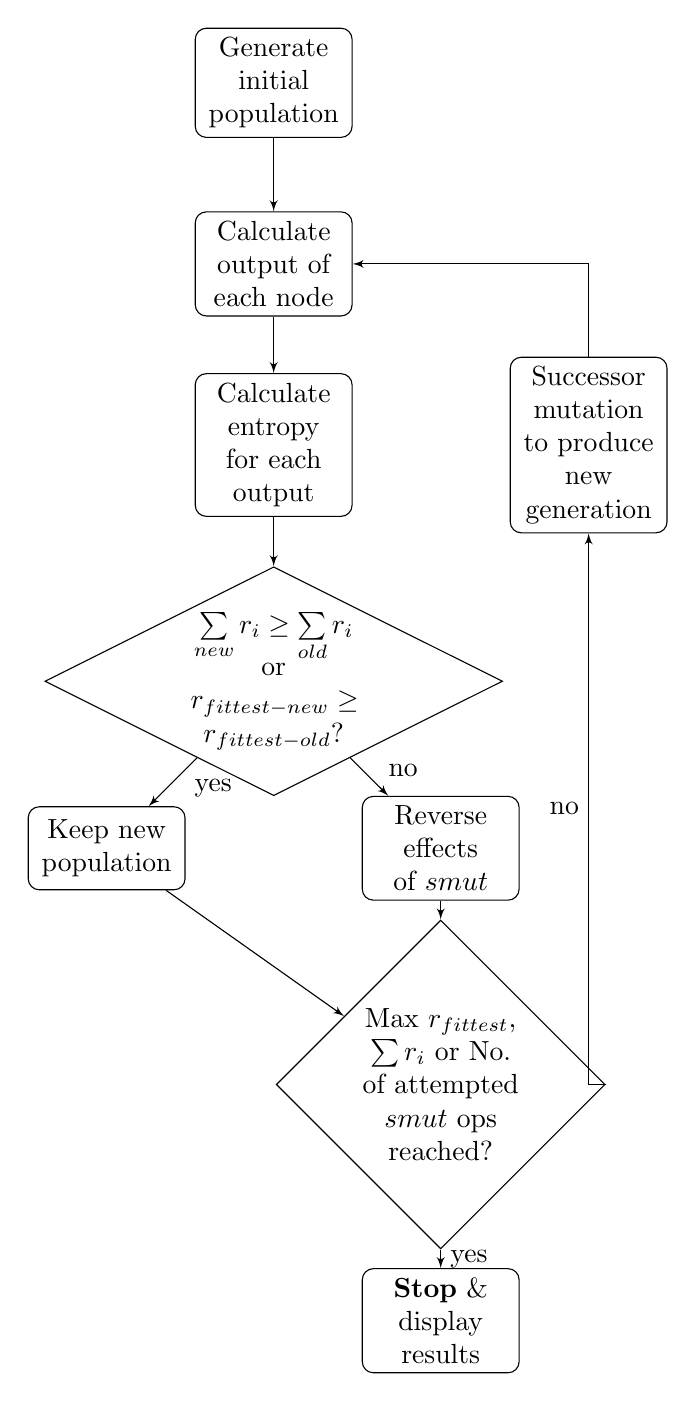
\begin{tikzpicture}[node distance = 2.3cm, auto]
    % Place nodes
    \node [block] (init) {Generate initial population};
    \node [block, below of=init] (identify) {Calculate output of each node};
    \node [block, below of=identify] (evaluate) {Calculate entropy for each output};
    \node [block, right of=evaluate, node distance=4cm] (update) {Successor mutation to produce new generation};
   
 \node [draw, decision, aspect=2,  below of=evaluate] (decide1) {$\sum\limits_{new} r_i \geq \sum\limits_{old} r_i$ or ${r}_{fittest-new} \geq {r}_{fittest-old}$?};
    \node [block, below left of=decide1, node distance=3cm] (greater) {Keep new population};
   \node [block, below right of=decide1, node distance=3cm] (less) {Reverse effects of $smut$};
    \node [decision, below of=less] (decide2) {Max $r_{fittest}$, $\sum r_i$ or No. of attempted $smut$ ops reached?};
    
\node [block, below of=decide2, node distance=3cm] (stop) {\textbf{Stop} \& display results};
    % Draw edges
    \path [line] (init) -- (identify);
    \path [line] (identify) -- (evaluate);
    \path [line] (evaluate) -- (decide1);
    \path [line] (decide1) -- node  [near start]{yes} (greater);
    \path [line] (decide1) -- node [near end] {no} (less);
    \path [line] (less) -- (decide2);
    \path [line] (greater) -- (decide2);
    \path [line] (decide2) -| node [near end] {no} (update);
    \path [line] (update) |- (identify);
    \path [line] (decide2) -- node {yes}(stop);
\end{tikzpicture}
\label{simpleflowsngp1}
\end{wrapfigure}



Figure \ref{simpleflowsngp1} shows a flowchart for the anticipated SNGP implementation. Here we can see that the main functions are similar to those of GP.
In SNGP, the initial population is also randomly generated but instead, members of the population are chosen as individual nodes.

The Inputs to the SNGP implementation are shown in figure \ref{inputparamsngp} on page \pageref{inputparamsngp}. There are less inputs for the SNGP implementation compared to the conventional GP implementation. The length of a run is the equivalent to the maximum number of generations for GP, where instead the program terminates after a certain number of attempted successor mutation operations. This has been changed since the original design document. Initially termination was designed to end on the number of successful $smut$ operations. It has since been changed to the number of attempted operations in order to bring fairness between GP and SNGP implementations. The terminating fitness value is taken from the sum of all fitness values in all the nodes of the population, or upon finding a solution (a root node representing a tree with an entropy greater than 27.990 bits). This has also been changed since the original design document, upon realisation that a single solution is desired. The population size is the number of nodes in the SNGP graph population. This size remains constant from initial generation throughout the rest of the run.

The SNGP population differs from the tree structure of a single member in the GP population. While the arity of functions and terminals remain the same as of that in the GP implementation, each function and terminal may have more than one predecessor. Therefore every node in the population can act as a root node for a RNG, and a population therefore contains as many RNGs as there are nodes. The reason for this coming about is due to the way that the population is initialised and evolved.

To begin with, all of the terminals in $T$ are added to the population exactly once. From here on in over all the generations, these terminals remain the same. What changes are their predecessors. Once the terminals are added, the functions are now selected randomly and are added to the population where their operands are existing members of the population. During initialisation of the population, the output and the fitness of each individual is also assessed. As Jackson describes in \cite[p.52]{jacksonsngp2}, this is what gives rise to SNGPs efficiency.

As the first terminals are added, they are evaluated for their outputs and their fitness is subsequently calculated. In this implementation of SNGP, this process is almost identical to that of the GP implementation described above. The terminal is evaluated for all values of $J$ from $i = 1$ to $2^{14}$, and each output is stored in the vector $O_i$ for that node. From this output vector a binary sequence of length $J$ is generated from the LSB of each element in $O_i$. The fitness of that node is the total entropy for subsequences of length 1 to 7 in the binary sequence, using the same equation as in the GP approach;
\begin{center}
 $E_{total} = \sum_{h = 1}^{7} \left[ - \sum_{j} P_{(hj)}\ \log_2\ P_{(hj)} \right]$
\end{center} 

This fitness/entropy value is stored in $r_i$ for that node. The efficiency of SNGP arises from using the following form of dynamic programming; when functions are now added to the population and their successors are assigned, the output and fitness for these nodes are calculated from the output vectors of their successors in the set $S_i$, as opposed to calculating them from scratch.

In SNGP, evolution is driven by hill-climbing. This is that the fitness is taken as the sum across the whole population; $\sum r_i$. After evolution this sum is calculated again, and if it is greater (higher entropy) than the last, then this evolved population replaces the previous population, otherwise the old population is kept and the process is repeated. I have changed the original design so that it is also driven on an increasing fittest member of the population. This way, it is easier to focus the evolution on trying to produce a solution as well as an entire graph with a high fitness. 

\begin{figure}[H]
\centering
\caption{Input parameters}
\label{inputparamsngp}
\begin{tabular}{l*{6}{l}r}
Data Type             & Input description\\
\hline
Integer & Length of a run (number of attempted $smut$ operations)\\
Integer & Population size (number of nodes)\\
Double & Total (i.e. sum of) target fitness value\\
\end{tabular}
\end{figure}

Evolution of a SNGP is not done by using the crossover operation like in the GP above, but instead uses the $smut$ or successor mutation operation. A member of the population (a node) is randomly selected, and one of the members in it's successor set is changed to another member of the population (still at a greater depth in the tree). 

During $smut$, not all of the program nodes are effected, and therefore not all of them need to be reevaluated for their outputs and fitnesses. As Jackson describes in \cite[p.53]{jacksonsngp} SNGP that retains it's efficient nature by creating an update list, where only nodes effected by smut are added. Nodes in the list are reevaluated starting at the lowest node in the list working up to the highest node so that no node is revisited.

The outputs for the SNGP implementation are almost identical to those of the GP. Instead of Generation Number, the output here will be the $smut$ operation count. Like the GP implementation I have also added the average fitness of the members of the population as an output. Please see the design document in the appendix for further detail on output data for the SNGP implementation.

Since the design document was produced, no changes have been made to the algorithms for the SNGP apart from the fitness function using the KMP matching algorithm, which is shown in algorithms \ref{fitnessfunc}, \ref{prefixfunc} and \ref{kmpalgo} in the design documents on pages \pageref{kmpalgo} and \pageref{fitnessfunc}. Please see the design document in the appendix for the algorithms specific to the SNGP implementation.

\textbf{Quick Evaluation Design}
\newpage
\section{Implementation / Realisation}
In this section I shall cover the transition I made from design into executable code. I shall cover the GP and SNGP implementations, as well as the program I produced in order to assess the C RNG and the TRNG at random.org.
- GP implementation, go through algorithms to code.\\
- SNGP implementation, go through algorithms to code.\\
- C rand() and TRNG test implementation. 
- Describe changes; KMP matching algorithm, SNGP update list order realisation, added run data collection, integer to long for calculations, change of driving evolution in SNGP, terminating on smut to attempted smut. \\
- Problems encountered, SNGP producing incorrect entropy values for some trees, 



\newpage
\section{Evaluation}

\subsection{Introduction}
%- Introduce how evaluation is based on collecting data from running all implementations and then comparing the results. Any part where running time factors into the analysis then AMD Athlon X2 5600+ 2.8GHz Dual core processor used. Explain changes to the test criteria from design document.\\
The first phase of evaluation is to compare the results I obtained from implementing Koza's method of producing randomisers with the use of Genetic Programming. By looking at the data he obtained and what I obtained, we should be able to paint an accurate picture of how well I managed to convey his description in his paper \cite{kozarng}.

A major (arguably the most important) part of this project is to evaluate the results produced by both GP and SNGP implementations. The aim is to prove which method of genetically breeding RNGs produces the most solutions in the most efficient manner (with respect to running time and the size of the solutions produced). 50 runs were conducted for both the single threaded GP and SNGP implementations in order to compare averages of their outputs. Runs used for any part of the following analysis where run time is taken into consideration were ran on a machine with an AMD Athlon 64 X2 5600+ 2.8 GHz Dual-Core processor.

The next step of evaluation after that is to compare the RNGs produced by the GP and SNGP paradigms against two other RNGs in wide use today. The C $rand()$ function is a PRNG that uses a Linear Congruent Generator algorithm in order to give developers who are writing C programs a simple way of generating pseudo random numbers. The Hardware/True Random Number Generator at random.org collects binary data from a radio receiver that reads atmospheric noise produced by unpredictable natural effects such as lightning storms. There is an API available where developers can download ``true" random data from the random.org servers for use in their software\footnote{Please see the implementation section of this document for details on how this is achieved}. 

Both of these methods of producing random numbers are analysed using the same technique in the fitness function in our GP \& SNGP implementations, by collecting 16834 random binary digits and calculating the Information Entropy for all possible binary subsequences of sizes 1 to 7 bits. These two methods of generating random numbers in both deterministic and non-deterministic ways give us two solid competitors for the random number generators produced by our evolutionary methods. 50 runs of these two implementations were also collected in order to compare entropy and scalar entropy break down against our genetically bred RNGs.

\subsection{Evaluation of GP Implementation}
%- Introduce evaluation by comparing first GP results to that of Kozas results. Compare any criteria that Koza proposes in his paper. Then show results and findings.\\

The first stage of implementation as discussed in the Realistion seciton of this document was to follow Koza's Paper \cite{kozarng} in implementing a GP to evolve RNGs in C. To do this, I developed algorithms\footnote{Found in the Design section of this document and in the design document in the appendix} that expressed the processes, equations and design in his paper. The first part of the evaluation is to assess the results that Koza produced against what I managed to acheive from the carbon copy of his implementation.

On pages \cite[p. 6 - 7]{kozarng}, Koza gives details of his results from one run, and that of several runs.
\subsection{50 Standard Runs: GP vs SNGP Implementation}
- Then introduce comparisons between GP and SNGP implementations under standard conditions for the 50 runs. Explain what will determine which method is most effective, i.e. minimal solution size, run time, highest fitness/entropy, highest solution rate, also average fitness of population increase of both. Then show results and findings and conclude to determine the victor.\\

\subsection{Parameter Altering Experimentation: GP vs SNGP Implementation}
- Introduce experimentation with the run conditions of both GP and SNGP. Then show results and findings.\\

\subsection{Genetic vs Conventional RNGs}
- Introduce comparisons of Genetic vs Conventional means of producing RNGs and random numbers.\\



\subsection{Temporary Graphs}

\begin{sidewaysfigure}[!]
\caption{Fittest RNG Tree - 27.995729 Bits  of Entropy}
\label{fulltree}
\resizebox{750pt}{!}{
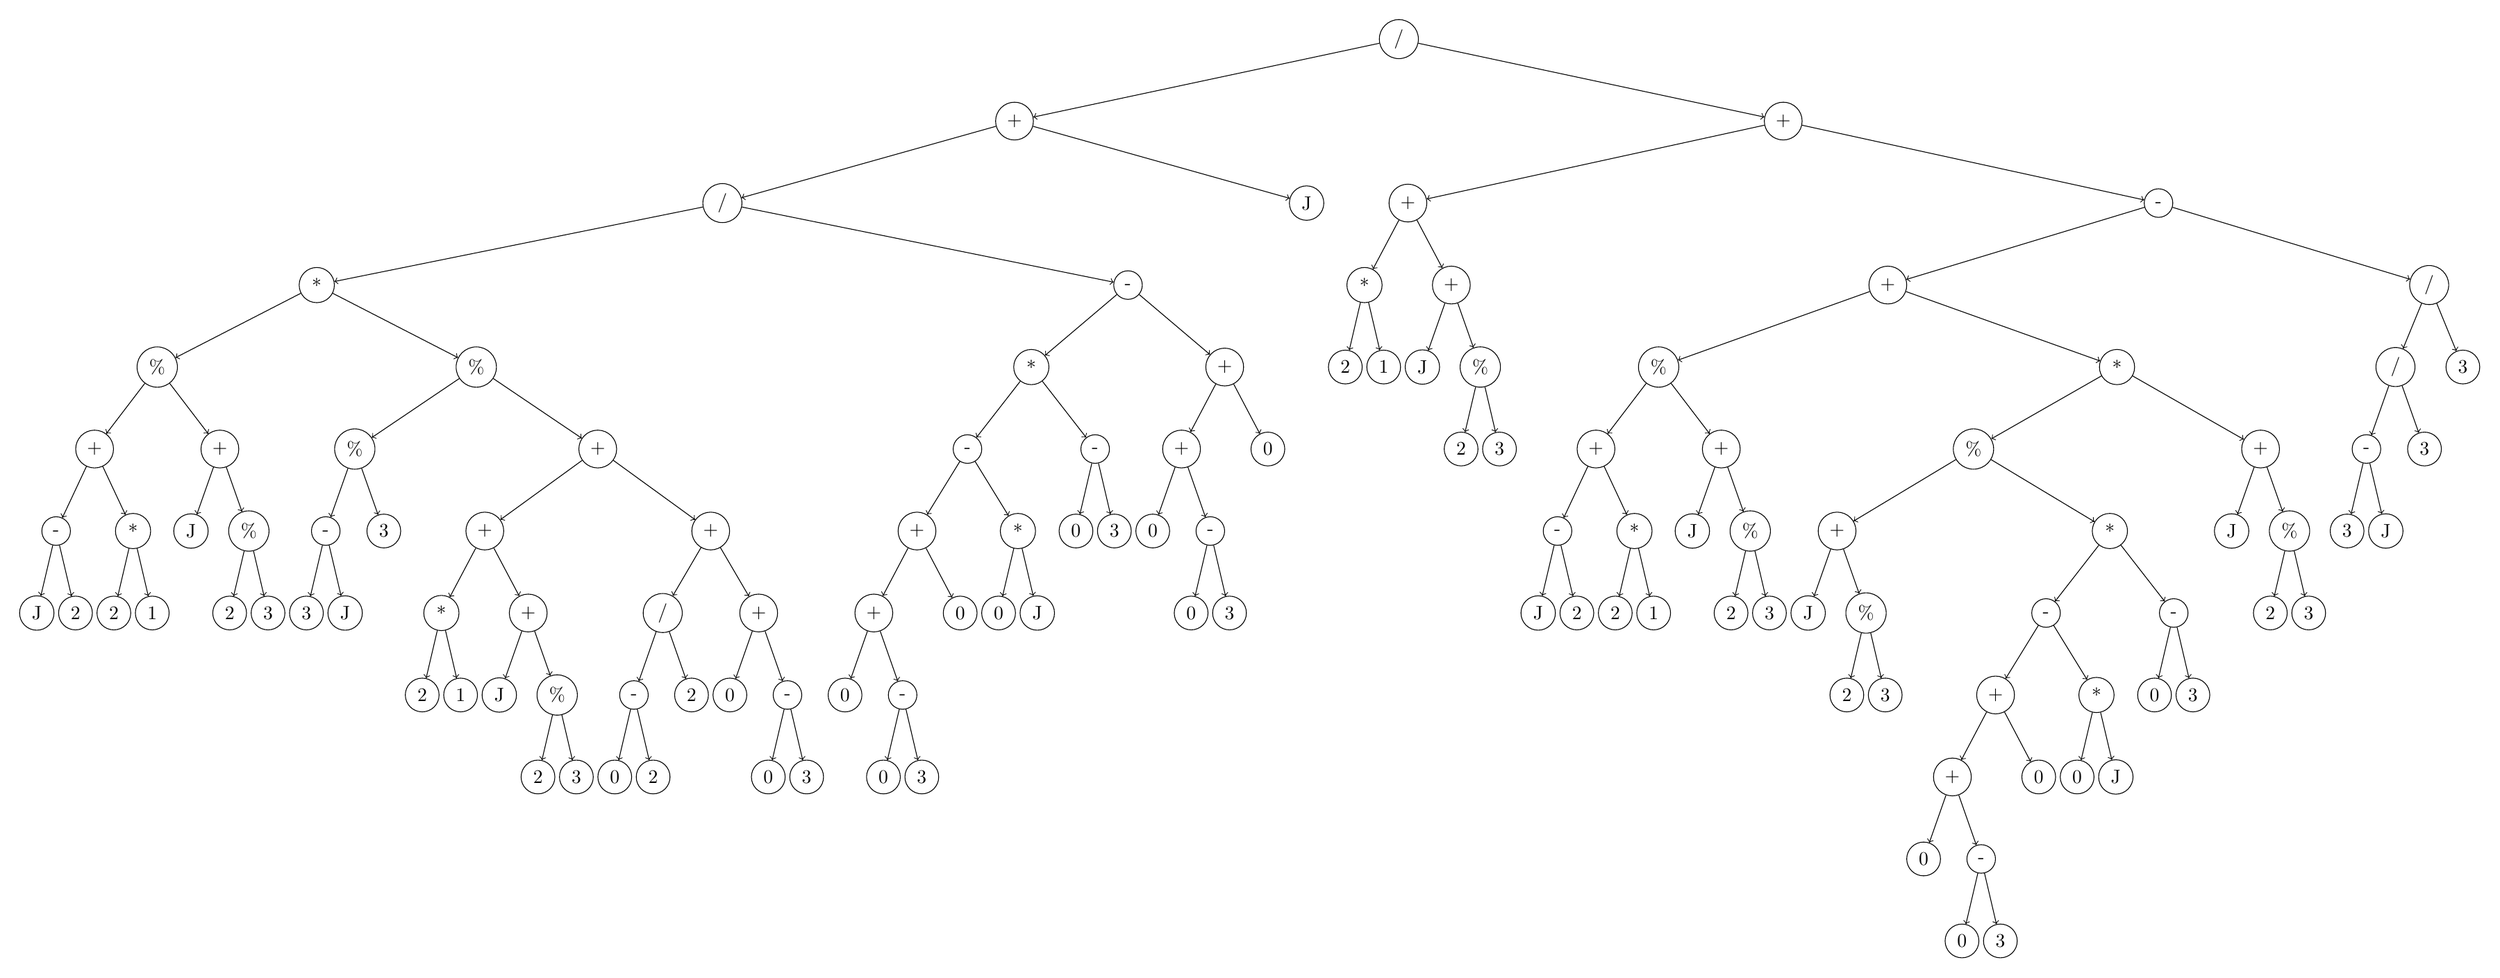
\begin{tikzpicture}[every tree node/.style={draw,circle,minimum size=1em}, level distance = 1.5cm,
edge from parent/.style={draw, ->, edge from parent path={(\tikzparentnode) -- (\tikzchildnode)}}]
\Tree[./ [.+ [./ [.* [.\% [.+ [.- J 2 ][.* 2 1 ]][.+ J [.\% 2 3 ]]][.\% [.\% [.- 3 J ]3 ][.+ [.+ [.* 2 1 ][.+ J [.\% 2 3 ]]][.+ [./ [.- 0 2 ]2 ][.+ 0 [.- 0 3 ]]]]]][.- [.* [.- [.+ [.+ 0 [.- 0 3 ]]0 ][.* 0 J ]][.- 0 3 ]][.+ [.+ 0 [.- 0 3 ]]0 ]]]J ][.+ [.+ [.* 2 1 ][.+ J [.\% 2 3 ]]][.- [.+ [.\% [.+ [.- J 2 ][.* 2 1 ]][.+ J [.\% 2 3 ]]][.* [.\% [.+ J [.\% 2 3 ]][.* [.- [.+ [.+ 0 [.- 0 3 ]]0 ][.* 0 J ]][.- 0 3 ]]][.+ J [.\% 2 3 ]]]][./ [./ [.- 3 J ]3 ]3 ]]]]
\end{tikzpicture}
}
\end{sidewaysfigure}
\newpage
\begin{figure}
\label{simplifiedtree}
\caption{Simplified RNG Tree}
\resizebox{500pt}{!}{
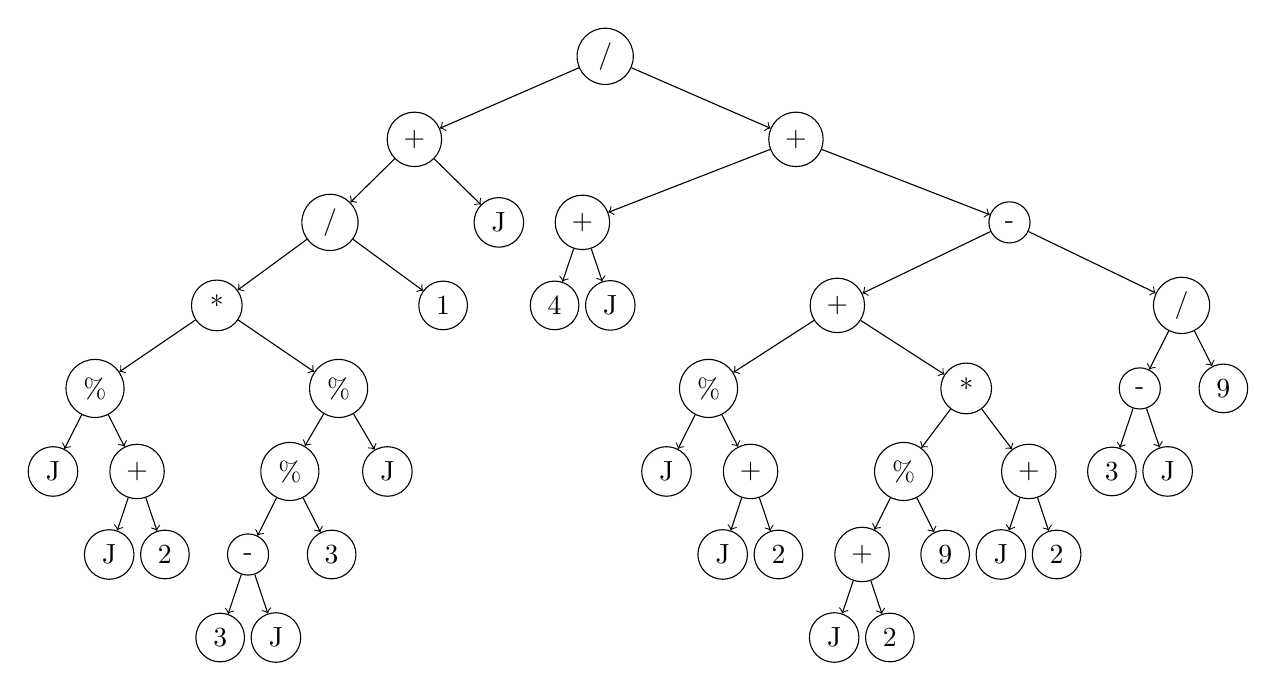
\begin{tikzpicture}[every tree node/.style={draw,circle,minimum size=1em},
edge from parent/.style={draw, ->,edge from parent path={(\tikzparentnode) -- (\tikzchildnode)}}]
\Tree[./ [.+ [./ [.* [.\% J [.+ J 2 ]][.\% [.\% [.- 3 J ]3 ]J ]]1 ]J ][.+ [.+ 4 J ][.- [.+ [.\% J [.+ J 2 ]][.* [.\% [.+ J 2 ]9 ][.+ J 2 ]]][./ [.- 3 J ]9 ]]]]
\end{tikzpicture}
}
\end{figure}
The RNG tree in figure \ref{fulltree} can be simplified by pre-calculating branches in the tree that operate only on constant values. When represented as an infix expression in a programming language, compliers will calculate this at compile time in order to reduce runtime in what's known as Constant Folding and Partial Redundancy Elimination. The tree in figure \ref{fulltree} can therefore be simplified into the tree in figure \ref{simplifiedtree}. This simplified tree can be represented as an infix mathematical function $f(J)$ below;
\begin{equation*}
f(J) = {{\left( (J\bmod (J+2))\ *\ (((3-J)\bmod 3)\bmod J) \over 12 \right) + J} \over {(4 + J) + \left((J\bmod(J+2) + ((J+2)\bmod 9) * (J+2)) - ({3-J \over 9}) \right)}}
\end{equation*}

\subsection{Real Implementation}
Another way to assess the successfulness of this project is to see the real world application of the RNGs produced by evolutionary methods. Take a smaller solution that was produced by the GP paradigm;

\begin{center}
/\ -\ 2\ -\ 2\ J\ \%\ J\ -\ 2\ /\ /\ J\ 3\ 3
\end{center}
This RNG achieved 27.995032 out of 28 bits of entropy. It can be represented as a mathematical function like so;

\begin{equation*}
rand(J) = {{(2 - ( 2 - J)} \over {J \mod (2 - \left({J \over 6}\right))}}
\end{equation*}
Remember that as discussed before, the RNGs are evolved on their binary output entropy and not as integer interpretation. Therefore in order to obtain integers with high entropy in an implementation, the RNG must create a stream of binary digits to then be interpreted as integers. They are also evolved based on their ability to randomise a sequence and not as a LCG. Therefore, in an implementation a seed value should be attained and then incremented in order to produce the best results. An example implementation of the function above can then be implemented in C code as seen below. 
\begin{lstlisting}[language=C, basicstyle=\small]
int randomiser(int min, int max) {
	max++; //Incrementing Max as to include it as a possible random output.
	int dec = 0;
	//Taking into account a negative minimum
	if (min < 0)
		max = (-1*min) + max;
	//Calculating the length of the stream we need
	int bit_max = (int) ceil(log10((double)max)/log10((double)2)); 
	//For that length we can read in the binary output of the random number generator
	for (int i = 0; i < bit_max; i++) {
		if ((protected_div(2 - (2 - seed), protected_mod(seed, (2 - (protected_div(protected_div(seed, 3), 3))))) % 2) == 1)
			dec = dec + pow((double)2, i);
		seed++; //Running through the sequence as we do.
	}
	//Returning the value between the defined range, taking into account a negative min
	int rand_return = 0;
	if (min < 0)
		rand_return = (dec % max) - (-1*min);
	else
		rand_return = ((dec % (max-min)) + min);
	return rand_return;
}
\end{lstlisting}
As discussed earlier the protected division and protected modulo functions return 1 if division or modulo by 0 is attempted.
This function can be seeded and called like so;

\begin{lstlisting}[language=C, basicstyle=\small]
int seed = time(NULL); //Seeded with the current time
int rand = randomiser(-300, 2000); //Generate a random number between -300 and 2000
\end{lstlisting}
Calling the randomiser function 100 times using the same parameters as seen above gave the following output;

\begin{lstlisting}[language=C, basicstyle=\small]
637  886  136  605  1256 393  555  213  969  715  290  1813 1429 557  26   1317 
1369 1441 157  -169 1668 689  -8   1028 429  1106 24   665  847  160  940  -144
-237 -215 1138 -235 286  1007 -86  1266 -225 1111 1518 -62  1023 984  1218 1235
1881 1788 1201 1903 -294 1244 1375 1258 380  1624 167  440  -141 1956 557  -273
778  495  1047 1288 706  1323 1908 1594 1076 665  1261 31   1432 1397 166  279
975  1195 1758 1084 932  658  84   408  400  168  420  337  72   -222 561  -122
485  -16  -154 792

\end{lstlisting}
Using this method, while producing a higher entropy result, is computationally more intensive than the C rand() function. This is because the RNG must be called $n$ times where $n$ is the number of bits required to reach the $max$ value defined by the user. This RNG can easily be parallelised however, so each RNG call can be done in parallel (because we can predict the seed values in advance). As we can see in figure \ref{rngcalls}, the running time of both the C rand() function and our genetically evolved RNG with respect to the number of calls on both are of the same order. However there exists some constant number of operations in our RNG implementation, that causes a longer over all running time. We can also see in figure \ref{rngmax} that over 1000 runs of each input, a higher value has no effect on the c rand() function, as the limit of the number is done with a simple modulus function. With our implementation of the genetically bred RNG, the max input size dictates how many bits we need and therefore how many calls of the RNG we need. Hence a larger max value has an effect on the running time (albeit small). We can conclude therefore that if an implementation of our RNG was desired by a developer, then a higher entropy output would come at the expense of computation time.

\begin{figure}[H]
%\centering
\begin{minipage}{.35\textwidth}
\caption{C $rand()$}
\includegraphics[keepaspectratio=true, height= 150pt]{crand.png}
\end{minipage}%
\begin{minipage}{.35\textwidth}
\caption{Random.org}
\includegraphics[keepaspectratio=true, height= 150pt]{randomorg.png}
\end{minipage}%
\begin{minipage}{.35\textwidth}
\caption{Genetic}
\includegraphics[keepaspectratio=true, height= 150pt]{myrand.png}
\end{minipage}%
\end{figure}

\begin{figure}[H]
\centering
\captionof{figure}{Logarithmic (base 10) Scale Run time of $n$ calls of $rand(J) = {{(2 - ( 2 - J)} \over {J \mod (2 - \left({J \over 6}\right))}}$ and C $rand()$, on the fixed min value of 0 and max value of 2000 for all runs}
\resizebox{350pt}{!}{
\begin{tikzpicture}
\label{rngcalls}
\begin{axis}[width=\textwidth, line width=2pt, grid=major,grid style={dashed}, ymax = 240, xmax = 10000000000, every axis label/.append style={font=\Large}, every tick label/.append style={font=\Large},
    xlabel={Number of Calls (n)},
    ylabel={Run Time (sec)}, smooth, xmode=log,
       log basis x={10}, legend style={
at={(0.55,0.34)},
anchor=north east},
enlarge x limits=false]
\addplot [color=lgreen] table [x=a, y=b, col sep=space, mark=none, smooth, color=lblue] {cvsmyrand.dat}  {};
\addplot [color=lorange] table [x=a, y=b, col sep=space, mark=none, smooth, color=lblue] {cvsmyrandc.dat}  {};

\legend{$rand(J) = {{(2 - ( 2 - J)} \over {J \mod (2 - \left({J \over 6}\right))}}$,C $rand()$}
\end{axis}
\end{tikzpicture}}
\end{figure}

\begin{figure}[H]
\centering
\captionof{figure}{Effect of increasing max value of random number on run time, 1000 calls for each max value. Logarithmic (base 10) Scale Run time of $rand(J) = {{(2 - ( 2 - J)} \over {J \mod (2 - \left({J \over 6}\right))}}$ and C $rand()$}
\resizebox{350pt}{!}{
\begin{tikzpicture}
\label{rngmax}
\begin{axis}[scaled ticks=false, tick label style={/pgf/number format/fixed}, width=\textwidth, line width=2pt, grid=major,grid style={dashed}, xmax = 10000000, every axis label/.append style={font=\Large}, every tick label/.append style={font=\Large},
    xlabel={Max value (n)},
    ylabel={Run Time (sec)}, smooth, xmode=log, ytick={0.00, 0.01,0.02,0.03,0.04,0.05,0.06},
       log basis x={10}, legend style={
at={(0.60,0.33)},
anchor=north east},
enlarge x limits=false]
\addplot [color=lgreen] table [x=a, y=b, col sep=space, mark=none, smooth, color=lblue] {rand_runtime.dat}  {};
\addplot [color=lorange] table [x=a, y=c, col sep=space, mark=none, smooth, color=lblue] {rand_runtime.dat}  {};

\legend{$rand(J) = {{(2 - ( 2 - J)} \over {J \mod (2 - \left({J \over 6}\right))}}$,C $rand()$}
\end{axis}
\end{tikzpicture}}
\end{figure}




\begin{figure}[H]
\centering
\begin{minipage}{.5\textwidth}
  \centering
\captionof{figure}{Reduced Pop size of SNGP}
\resizebox{220pt}{!}{
\begin{tikzpicture}
\begin{axis}[width=\textwidth, line width=2pt, grid=major,grid style={dashed}, ymax = 100, ymin = 0, xmin = 0, xmax = 100, every axis label/.append style={font=\Large}, every tick label/.append style={font=\Large},
    xlabel={Population Size},
    ylabel={Solution Rate (\%)}, smooth,  xtick={0,20,40,60, 80, 100},
stack plots=y,
enlarge x limits=false]
\addplot [color=lblue] table [x=a, y=b, col sep=space, mark=none, smooth, color=lblue] {sngpreduced.dat}  {};
\end{axis}
\end{tikzpicture}}
\end{minipage}%
\begin{minipage}{.5\textwidth}
  \centering
\captionof{figure}{Reduced Pop size of GP}
  \resizebox{220pt}{!}{
\begin{tikzpicture}
\begin{axis}[width=\textwidth, line width=2pt, grid=major,grid style={dashed}, ymax = 100, ymin = 0, xmin = 0, xmax = 500, every axis label/.append style={font=\Large}, every tick label/.append style={font=\Large},
    xlabel={Population Size},
    ylabel={Solution Rate (\%)}, smooth,  xtick={0,100,200,300,400, 500},
stack plots=y,
enlarge x limits=false,]
\addplot [color=lred] table [x=a, y=b, col sep=space, mark=none, smooth, lred] {gpreduced.dat}  {};
\end{axis}
\end{tikzpicture}}
\end{minipage}
\end{figure}
\section{Learning Points}
At least one page of summary of the key learning points in the project.
\section{Professional Issues}
At least one page of discussion of how your project related to the codes of practice and conduct issued by the British Computer Society.



%\begin{figure}[H]
%\centering
%\begin{minipage}{.5\textwidth}
 % \centering
%\captionof{figure}{Run time of $rand(J) = {{(2 - ( 2 - J)} \over {J \mod (2 - \left({J \over 6}\right))}}$}
%\resizebox{220pt}{!}{
%\begin{tikzpicture}
%\label{randruntime}
%\begin{axis}[width=\textwidth, line width=2pt, grid=major,grid style={dashed}, every axis label/.append style={font=\Large}, every tick label/.append style={font=\Large},
%    xlabel={Input size(n)},
  %  ylabel={Run Time (sec)}, smooth, 
%stack plots=y,
%enlarge x limits=false]
%\addplot [color=lgreen] table [x=a, y=b, col sep=space, mark=none, smooth, color=lblue] {cvsmyrand.dat}  {};
%\end{axis}
%\end{tikzpicture}}
%\end{minipage}%
%\begin{minipage}{.5\textwidth}
 % \centering
%\captionof{figure}{Run time of C $rand()$ function}
%  \resizebox{220pt}{!}{
%\begin{tikzpicture}
%\label{cruntime}
%\begin{axis}[width=\textwidth, line width=2pt, grid=major,grid style={dashed}, every axis label/.append style={font=\Large}, every tick label/.append %style={font=\Large},
%    xlabel={Input size(n)},
%    ylabel={Run Time (sec)}, smooth, 
%enlarge x limits=false]
%\addplot [color=dorange] table [x=a, y=c, col sep=space, mark=none, smooth, lred] {cvsmyrand.dat}  {};
%\end{axis}
%\end{tikzpicture}}
%\end{minipage}
%\end{figure}


















\section{Bibliography}
\begin{thebibliography}{11}

\bibitem{kozarng}
  John R. Koza, 
  \emph{Evolving a Computer Program to Generate Random Numbers Using the Genetic Programming Paradigm}. 
  Stanford University, 
  1991.

\bibitem{jacksonsngp}
  David Jackson,
  \emph{Single Node Genetic Programming on Problems with Side Effects}.
  University of Liverpool,
  2012.

\bibitem{nist}
  Andrew Rukhin, Juan Soto, James Nechvatal, Miles Smid, Elaine Barker, Stefan Leigh, Mark Levenson, Mark Vangel,David Banks, Alan Heckert, James Dray, San Vo 
  \emph{A Statistical Test Suite for Random and Pseudorandom Number Generators for Cryptographic Applications}. 
  NIST,
  2010.

\bibitem{mitchell}
  Melanie Mitchell,
  \emph{An Introduction to Genetic Algorithms}.
  MIT Press,
  1999.

\bibitem{lapantebio}
  Phillip A. Laplante,
  \emph{Biocomputing}.
  Nova Science Publishers Inc,
  2003.

\bibitem{introgp}
  R. Poli, W. B. Langdon, N. F. McPhee, J. R. Koza, 
  \emph{A Field Guide to Genetic Programming}. 
  University of Essex, 
  2008.

\bibitem{kozagpbook}
  John R. Koza, 
  \emph{Genetic Programming. On the Programming of Computers by Means of Natural Selection}. 
  MIT Press, 
  1992.

\bibitem{kozamux}
  John R. Koza,
  \emph{A Hierarchical Approach to Learning the Boolean Multiplexer Function}
  Stanford University,
  1990.

\bibitem{cprog}
  Brian W. Kernighan, Dennis M. Ritchie, 
  \emph{C Programming Language}.
  2nd Edition, 
  Prentice Hall Professional Technical Reference, 
  1988.

\bibitem{jacksonsngp2}
  David Jackson,
  \emph{A New, Node-Focused Model for Genetic Programming}.
  Proceedings of the 15th European Conference on Genetic Programming, EuroGP 2012, 
  Springer Verlag
  2012.

\bibitem{prnggp}
  C. Lamenca-Martinez, J.C. Hernandez-Castro,
  J.M. Estevez-Tapiador, and A. Ribagorda
  \emph{Lamar: A New Pseudorandom Number Generator Evolved by means of Genetic Programming}.
  University of Madrid,
  2006.

\bibitem{entropy}
  Robert M. Gray
  \emph{Entropy and Information Theory}.
  First Edition (Corrected),
  Stanford Unviersity
  2000.

\end{thebibliography}

\section{Appendices}
Appendices are meant to contain detailed material, required for completeness, but which are too detailed to include in the main body of the text. Typically they should contain code listings, details of test data, screen shots of sample runs, a user guide, full design diagrams, instructions for unpacking and mounting any software included with the dissertation and similar material. A disc or CD-ROM containing the project archive material (including source codes, pictures used, and the dissertation document) should be submitted with the project report. Instructions on how to run the software from the disc/CD-ROM should be provided. If your system is available on-line, you should provide instructions of how to access the system via the internet.
\end{document}